%!TEX root=main.tex
\section{引言}
\label{kvdirect:sec:introduction}

本章的主题是存储虚拟化与数据结构处理加速,在全文中的位置如图 \ref{kvdirect:fig:sys-arch} 所示。

\begin{figure}[htbp]
	\centering
	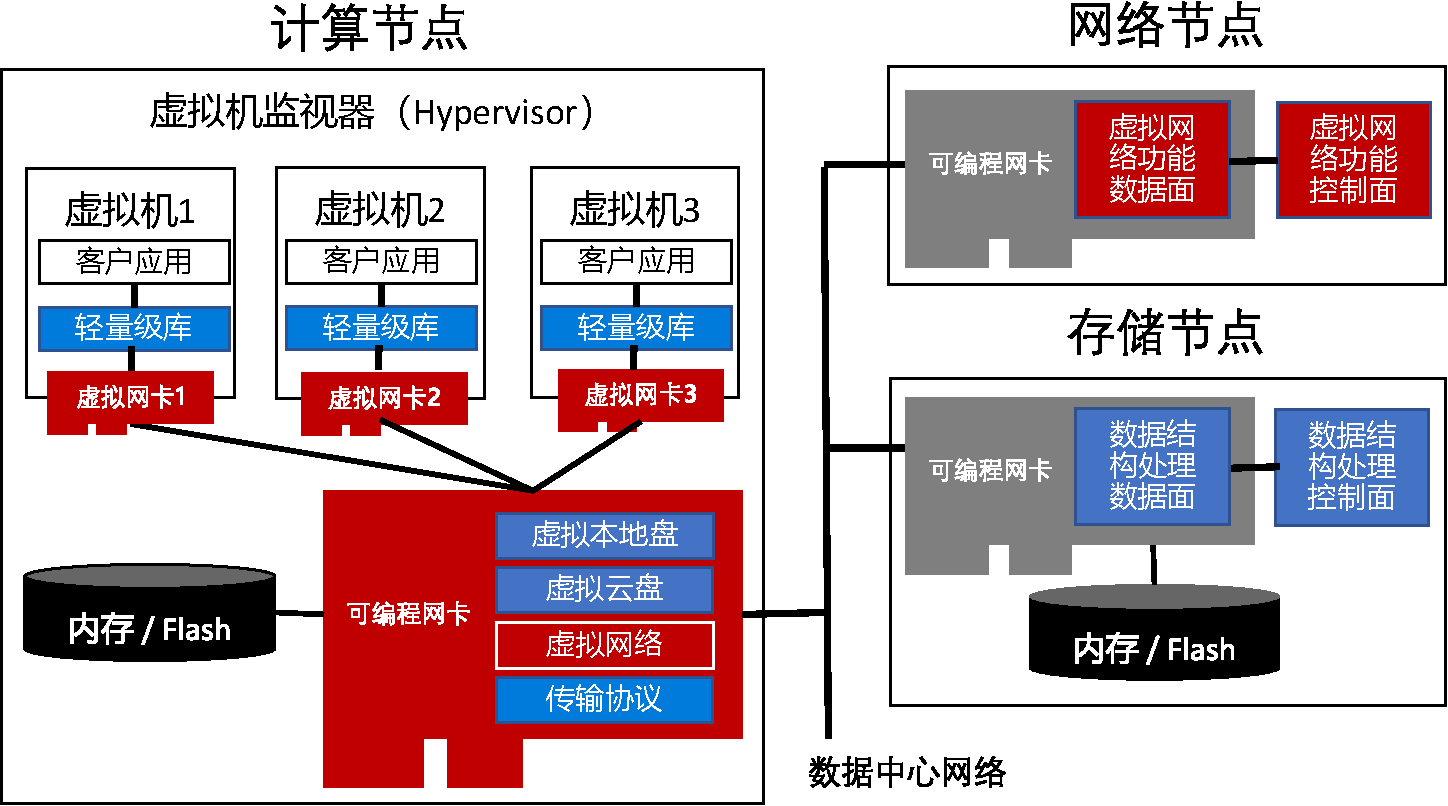
\includegraphics[width=0.8\textwidth]{figure/sys_arch.pdf}
	\caption{本章主题:存储虚拟化与数据结构处理加速,用红色标出。}
	\label{kvdirect:fig:sys-arch}
\end{figure}

在可编程网卡的编程方面,本章基于上一章提出的 ClickNP 编程框架,搭建了服务层的基础,提出了有状态处理和数据结构处理的框架,并基于此实现了内存键值存储,如图 \ref{kvdirect:fig:sw-hw-codesign} 所示。

\begin{figure}[htbp]
	\centering
	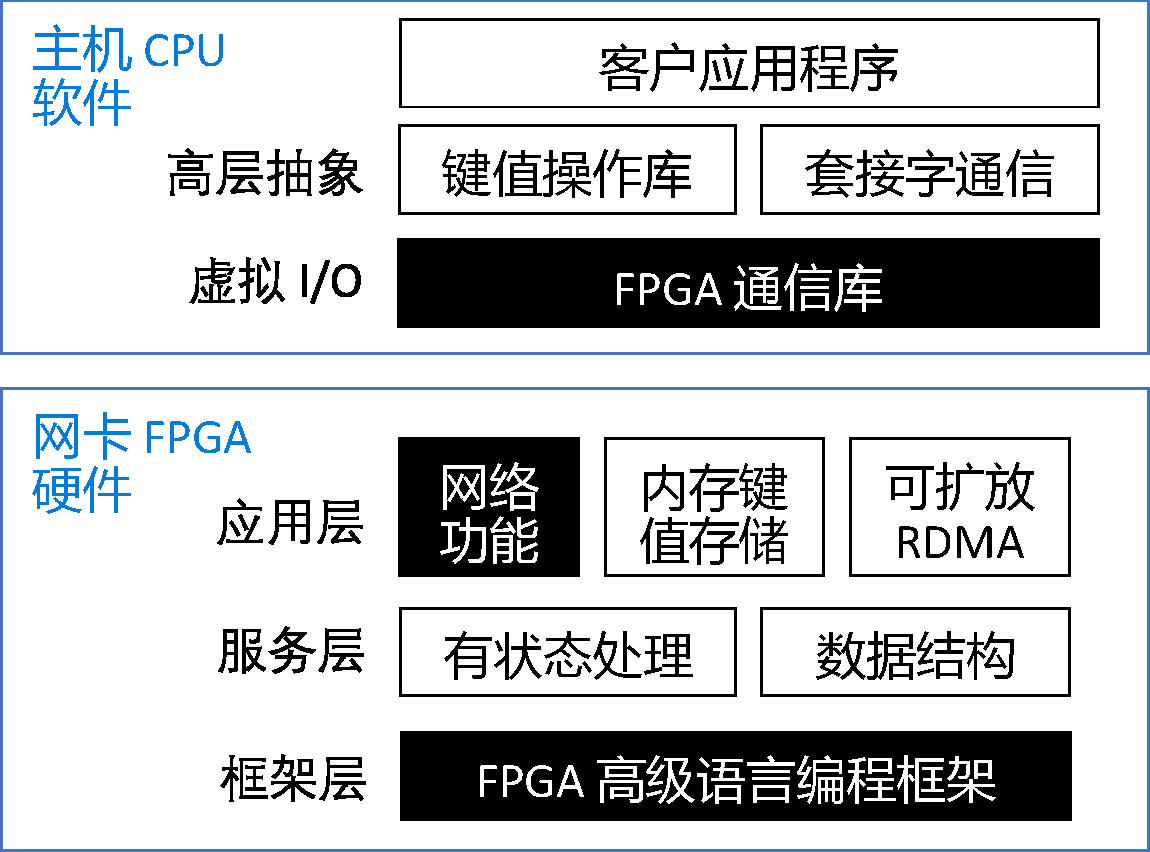
\includegraphics[width=0.5\textwidth]{figure/sw_hw_codesign.pdf}
	\caption{本章在可编程网卡软硬件架构中的位置。}
	\label{kvdirect:fig:sw-hw-codesign}
\end{figure}


%\subsection{outline}
%
%键值 is an important infrastructure service
%
%Existing solution of key-value store in
%
%1. CPU-based
%
%2. RDMA-based
%
%recent trend of programmable 网卡 in datacenter
%
%we present 键值-Direct... 
%
%highlight the high level insight (offload the simple and performance critical operation to programmable 网卡) 
%
%and design goal and spotlight (not only match the state of art of RDMA-based solution in GET operation and significant improve the PUT operation to even comparable to CPU-based solution. Moreover, our solution is more power and cost effective. With more FPGA or the improvement of FPGA, we can beat all existing CPU/RDMA solution.)
%
%键值-Direct makes contributions in three main aspects:
%
%1. proposes a 键值 solution for programmable 网卡 to Direct Memory Access.
%
%2. extends RDMA primitives to Key-value operation with consistency guarantee while high performance. 
%
%3. makes critical PCIe traffic optimization in our novel FPGA-based 网卡 key-value service design.



%Key-value store (键值存储) is an infrastructure service to store shared structured data in a distributed system.
%Traditionally, the performance of 键值存储 is mostly constrained by the OS network stack.
%Recent research leverage two-sided RDMA to accelerate communication among clients and 键值存储 servers.
%The next bottleneck is CPU. The 键值 operation throughput of a CPU core is constrained by its latency hiding efficiency and computation capacity.
%Another approach is to use one-sided RDMA to bypass remote CPU and move 键值 processing to clients, but it incurs high communication and synchronization overhead.
%\subsection{current version}



\begin{figure*}[t]
\centering
\subfloat[软件 / 双侧 RDMA。\label{kvdirect:fig:memaccess-a}]
{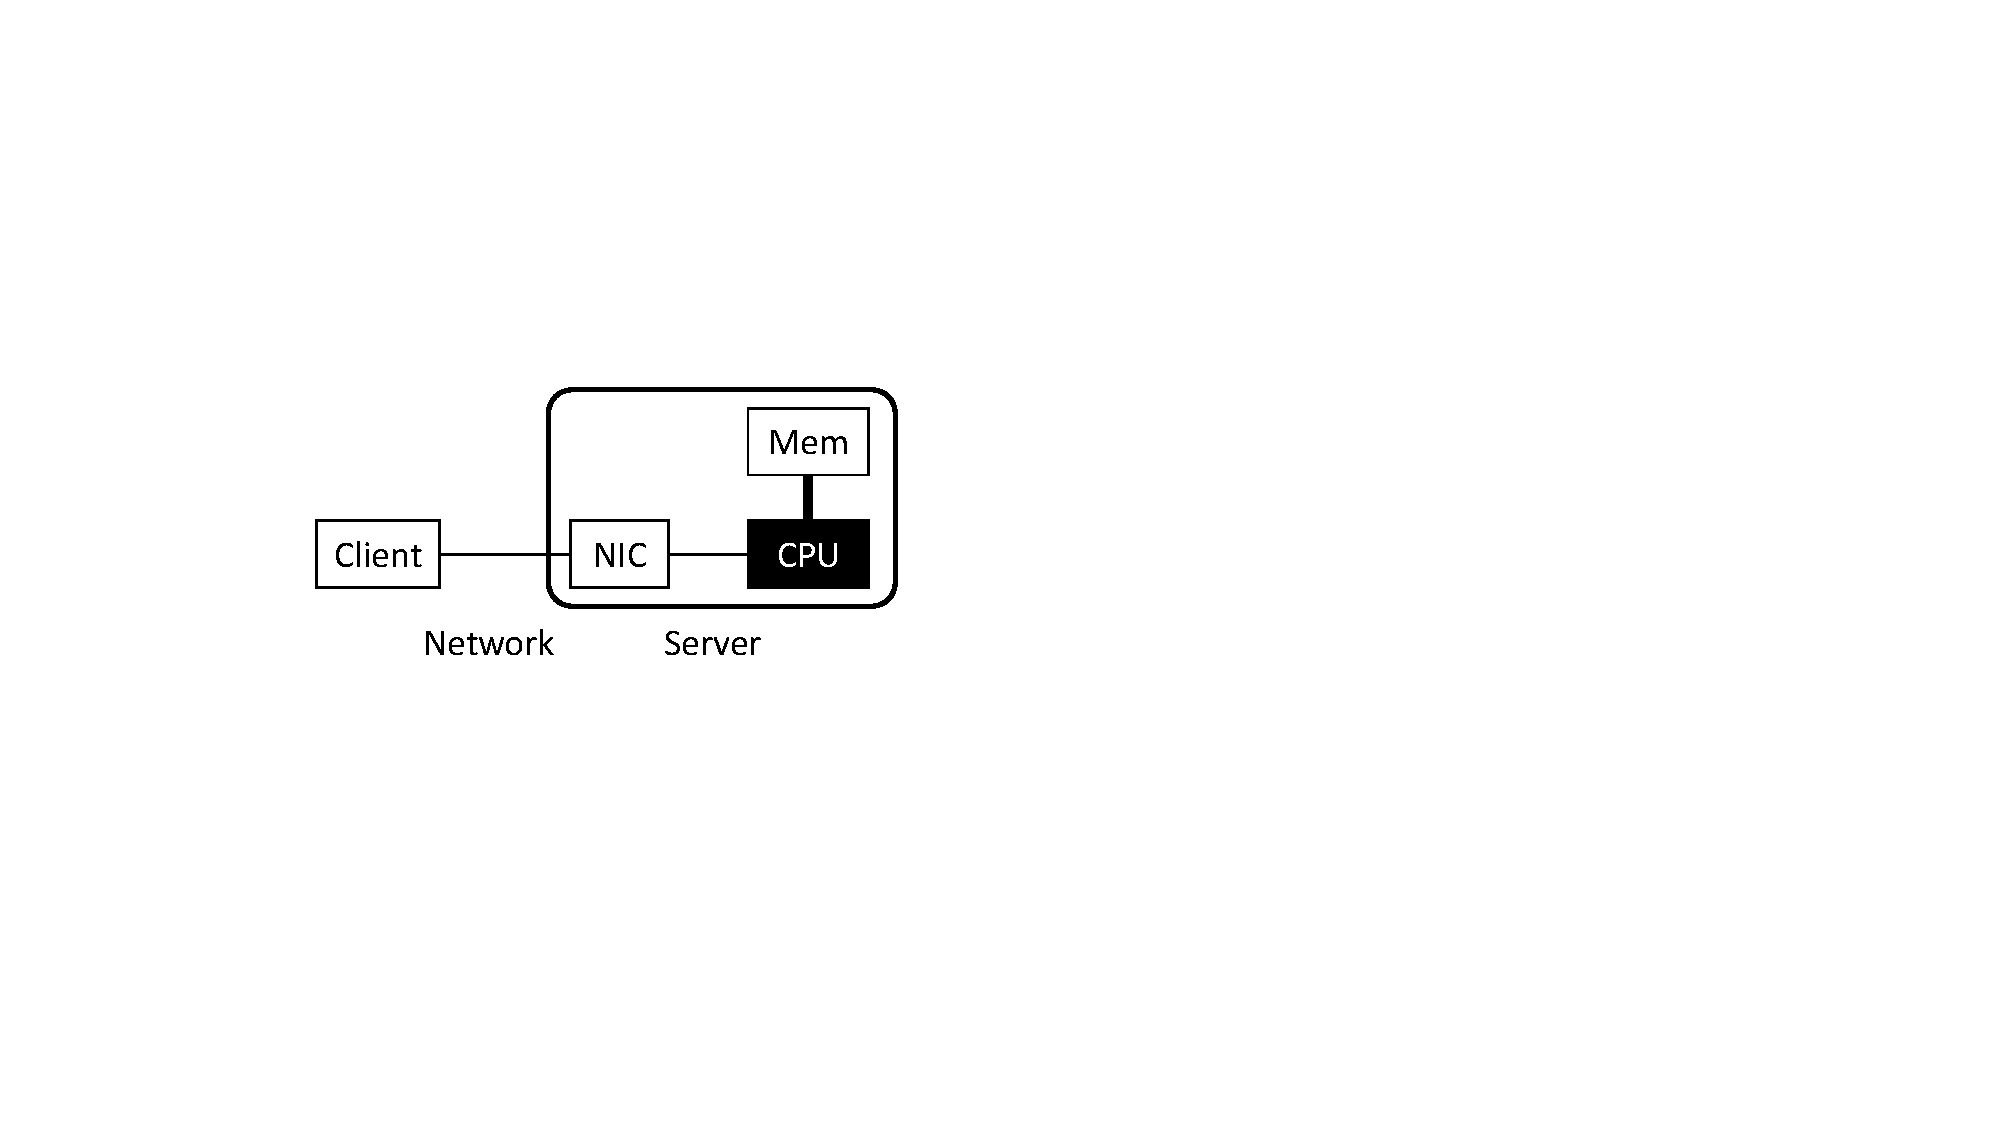
\includegraphics[width=.33\textwidth,page=1]{cropped_access.pdf}}
\subfloat[单侧 RDMA。\label{kvdirect:fig:memaccess-b}]
{\includegraphics[width=.33\textwidth,page=2]{cropped_access.pdf}}
\subfloat[\oursys{}。\label{kvdirect:fig:memaccess-c}]
{\includegraphics[width=.33\textwidth,page=3]{cropped_access.pdf}}
\caption{键值存储数据通路和处理装置的设计空间。 行表示数据路径。 一个键值操作(细线)可能需要多个基于地址的存储器访问(粗线)。 黑框表示键值处理发生的位置。}
\label{kvdirect:fig:memaccess}
\end{figure*}

内存中键值存储(键值存储)是许多数据中心中的关键分布式系统组件。 键值存储允许在分布式客户端之间访问共享键值哈希表。从历史上看,诸如Memcached \cite {fitzpatrick2004distributed}之类的键值存储作为Web服务的对象缓存系统获得了普及。亚马逊\cite {decandia2007dynamo}和Facebook \cite {atikoglu2012workload,nishtala2013scaling}等大型网络服务提供商已大规模部署了分布式键值存储。最近,随着基于主内存的计算成为数据中心的一个主要趋势 \cite{ousterhout2010case,dragojevic2014farm},键值存储开始超越缓存并成为在分布式系统中存储共享数据结构的基础架构。

许多数据结构可以在键值哈希表中表示,例如,NoSQL数据库中的数据索引\cite {chang2008bigtable},机器学习中的模型参数\cite {li2014scaling},图形计算中的节点和边缘\cite {shao2013trinity,xiao17tux2}和分布式同步中的序列发生器\cite {kalia2016design}。对于大多数这些应用,键值存储的性能是直接决定系统效率的关键因素。由于其重要性,多年来已投入大量研究工作来改善键值存储性能。

早期的键值系统\cite {decandia2007dynamo,fitzpatrick2004distributed,nishtala2013scaling} 建立在传统操作系统抽象的基础之上,例如OS锁和TCP / IP堆栈。这给操作系统的性能带来了相当大的压力,尤其是网络堆栈。由于数据中心应用带宽需求过大,物理网络传输速度在过去十年中有了巨大的改进,这加剧了瓶颈。

最近,随着单核频率提升和多核架构扩展速度的减慢,分布式系统的一项新研究趋势是利用网卡上的远程直接内存访问(RDMA)技术来减少网络处理成本。一系列研究\cite {kalia2014using,kalia2016design}使用双面RDMA加速通信(图\ref {kvdirect:fig:memaccess-a})。使用这种方法构建的键值存储受到键值存储服务器的CPU性能的限制。另一系列研究使用单侧RDMA绕过远程CPU并将键值处理工作量转移到客户端\cite {dragojevic2014farm,mitchell2013using}(图\ref {kvdirect:fig:memaccess-b})。这种方法实现了更好的GET性能,但由于高通信和同步开销,降低了PUT操作的性能。由于缺乏事务支持,RDMA提供的抽象不适合构建高效的键值存储。

与此同时,数据中心硬件发展的另一个趋势正在出现。数据中心中越来越多的服务器现在配备了可编程网卡 \cite{caulfield2016cloud,greenberg2015sdn,putnam2014reconfigurable}。
可编程网卡的核心是现场可编程门阵列(FPGA),其具有用于连接到网络的嵌入式网卡芯片和用于连接到服务器的PCIe连接器。
可编程网卡最初设计用于启用网络虚拟化\cite {vfp,li2016clicknp}。
但是,许多人发现FPGA资源可以用来卸载CPU的一些工作负载,并显着降低CPU资源的使用量\cite {ouyang14hotchips,MaZC17fpga,huang16socc,cong16dac}。我们的工作采用这种一般方法。

我们提出\oursys{},一个新的内存中键值系统,利用数据中心的可编程网卡。
顾名思义,\oursys{} 直接获取数据并在主机内存中应用更新来为键值请求提供服务,绕过主机CPU(图 \ref {kvdirect:fig:memaccess-c})。
我们利用单侧基于RDMA的键值系统的洞察力来绕过CPU,同时将计算逻辑卸载到基于FPGA的网卡,以确保服务器端的一致性,从而通过减少网络流量和减少同步开销实现显着的性能提升此外,客户端对所有键值操作都变得透明。
\oursys{} 将RDMA原语从内存操作(READ和WRITE)扩展到键值操作(GET,PUT,DELETE和ATOMIC操作)。与基于单面RDMA的系统相比,\oursys{} 处理服务器端的一致性和同步问题,从而消除了客户端的计算负荷并减少了网络流量。
此外,为了支持基于矢量的操作并减少网络流量,\oursys{} 还提供了新的矢量原语UPDATE,REDUCE和FILTER,允许用户定义活动消息(active message)\cite {eicken1992active}并将某些计算委托给可编程网卡。

由于键值操作已卸载到可编程网卡,因此我们将设计重点放在优化网卡和主机内存之间的PCIe流量上。 \oursys{} 采用一系列优化来充分利用PCIe带宽和隐藏延迟。首先,我们设计了一个新的哈希表和内存分配器,以利用FPGA中可用的并行性,并最大限度地减少PCIe DMA请求的数量。平均而言,\oursys{} 每次READ操作接近一个PCIe DMA,每个WRITE操作两个PCIe DMA。其次,为了保证从属键值操作之间的一致性,\oursys{} 包括一个无序执行引擎来跟踪操作依赖性,同时最大化独立请求的吞吐量。第三,\oursys{} 通过在FPGA中实现基于硬件的负载调度程序和缓存组件来充分利用板载DRAM带宽和容量,利用可编程网卡上可用的板载DRAM缓冲区。

单网卡 \oursys{} 系统能够实现每秒高达180~M 键值的操作(Ops),相当于36个CPU核心的吞吐量\cite {li2016full}。与最先进的CPU 键值存储实现相比,\oursys{} 可将尾延迟降低至10 $\mu$s,同时将功率效率提高3倍。而且,\oursys{} 可以通过多个网卡实现接近线性的可扩展性。在服务器中使用10个可编程网卡,我们在单个商品服务器中每秒实现12.2亿键值操作,这比现有系统提高了一个数量级。

\oursys{} 支持高达180~Mops的一般原子操作,等于正常的键值操作,并且明显优于最先进的基于RDMA的系统中报告的数量:2.24~Mops \cite {kalia2014using}。原子操作的性能主要是我们的乱序执行引擎的结果,该引擎可以有效地跟踪键值操作之间的依赖性,而不会阻塞管道。

本章的其余部分安排如下。 \S \ref {kvdirect:sec:background}显示了背景,阐明了我们的设计目标和挑战。 \S \ref {kvdirect:sec:architecture}描述了\oursys{} 的设计。 \S \ref {kvdirect:sec:implementation}显示了\oursys{} 的实现细节。 \S \ref {kvdirect:sec:evaluation}是对\oursys{} 的评估。 \S \ref {kvdirect:sec:extensions}讨论了进一步的扩展。 我们在\S \ref {kvdirect:sec:related}中讨论相关工作,并在\S \ref {kvdirect:sec:conclusion}中得出结论。
